\chapter{Physical introduction}
Most parts of this chapter are inspired by \citep{kolodrubez} and original notes \citep{berry1984}, \citep{berry1989}, \citep{berry2009}
Now we will assign some physical background to the structure defined in the first chapter.

Assume manifold $\M$ generated by eigenstates of some closed system Hamiltonian $\HH(\llambda)$, meaning the Hamiltonian is bounded and dimension of the space is finite. This is truly manifold, because there exists $\mathcal{C}^1$ mapping\footnote{is continuous to the first derivative} $B: \M\rightarrow \bm\llambda\equiv (\lambda^1,\dots,\lambda^n)\in\R^n$. Hamiltonian finitedimentinality implies, that the spectrum is discrete at any point $\llambda$, thus $\sigma=\{\ket{n(\bm\llambda)}\}_n$ with energies $E_n(\bm\llambda)$. 
\citep{berry1984} The state of the system evolves according to \Schrodinger equation
\begin{equation}
    i\hbar \d_t\kpsit = \HH(\llambda(t))\kpsit,
    \label{eq:schrodinger}
\end{equation}
which for eigenstates reads as
\begin{equation}
    \HH(\llambda(t))\ket{n(\llambda(t))}=E_n(\llambda(t))\ket{n(\llambda(t))}.
    \label{eq:energySchrodinger}
\end{equation}
Geometrical meaning of changing parameter $\llambda$ can be understood as parallel transport of vectors along some curve $\gamma=\{\gamma(t)| t\in[0,T]\}$ on $\M$, which gives
\begin{equation}
    \Par_\gamma \ket{n} = \ket{\tilde n}.
\end{equation}
To get some geometrical intuition, see fig. \ref{fig:manifoldIntuition}.

\begin{figure}[h]
    \centering
    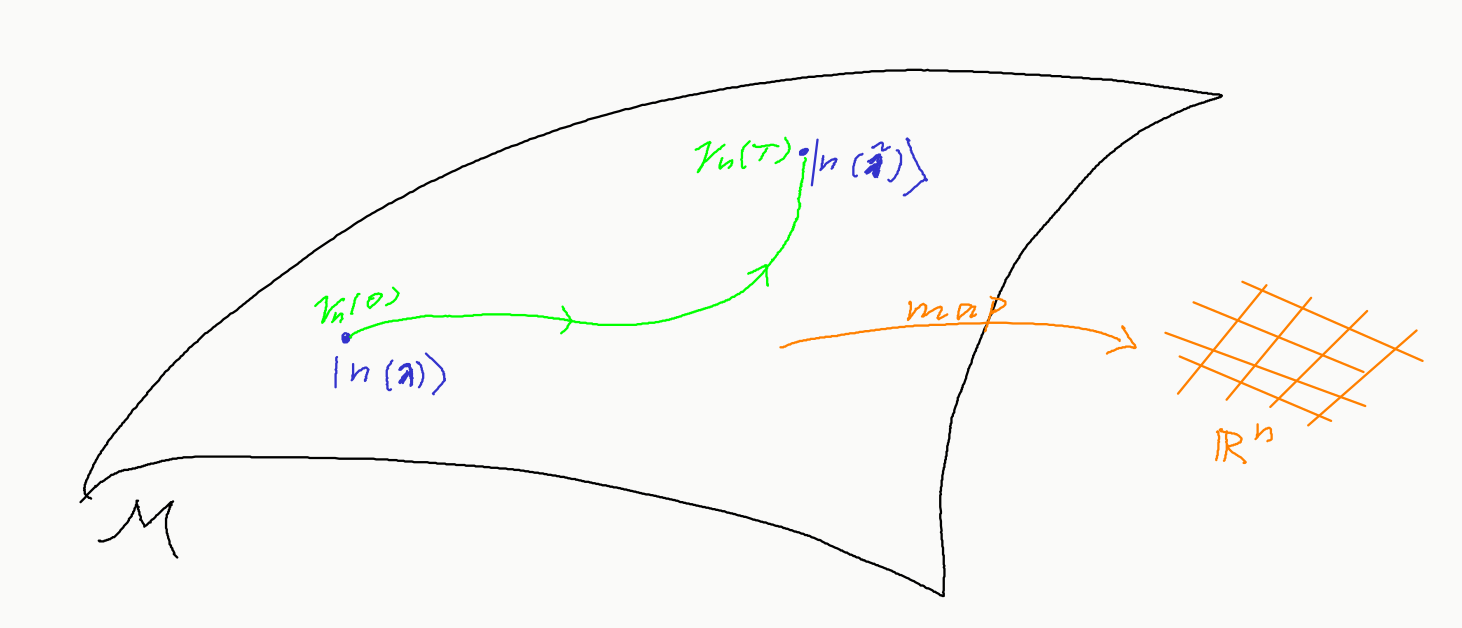
\includegraphics[width=0.8\textwidth]{../img/manifoldIntuitionTransport.png}
\caption{Manifold $\M$ defined by Hamiltonian $\H(\llambda)$, where at every point we can construct tangent space as a defining space for clear quantum states, i.e. can be constructed as superposition of eigenstates. This can be parallelly transported to some other point using $\gamma$.}
    \label{fig:manifoldIntuition}
\end{figure}


To parallelly transport states, it is sufficient to transport it's basis using $\gamma_n(\xi)$. The solution to eq. \ref{eq:energySchrodinger} is then
\begin{equation}
    \kpsit \equiv \Par_{\gamma_n}\ket{n} = \exp\left(-\frac{i}{\hbar}\int_0^tE_n(\llambda(\tau)\d\tau)\right)\exp(i\gamma_n(t))\ket{n(\llambda(t))}.
    \label{eq:phasesOnManifold}
\end{equation}
The first exponential, the \emph{dynamical phase}, is well known if we switch of the dependence on $\llambda$ and depend only on time and energy of states during the transport. The second exponential is called \emph{geometrical phase}. This phase is generally non-integrable, meaning it cannot be written simply as $\gamma_n(\llambda(t))$ and for some closed curve on $\M$
\begin{equation}
    C=\{\llambda(\xi)|\xi\in[0,\Xi] \text{, such that }\llambda(0)=\llambda(\Xi)\}
\end{equation} 
we generally get $\Par_C \psi(\llambda)\neq \psi(\llambda)$. This property is sometimes more generally called \emph{anholonomy} and should be defined properly.
\begin{definition}[Anholonomy]
    Geometrical phenomenon, which causes some variable $V(\gamma(p))$ not to return to it's original value while varying it's parameter $p$ around some closed curve $\gamma(p)$. 
\end{definition}
If the transporting variable is quantum state, we can measure some non-zero angle between $\ket{V(\gamma(0))}$ and $\ket{V(\gamma(p))}$, whilst $\gamma(p)=\gamma(0)$, meaning
$$\braket{V(\gamma(0))|V(\gamma(p))}\neq 0.$$ 
The geometric intuition of anholonomy can be seen on fig. \ref{fig:parallelTransportClosed}.

\begin{figure}[h]
    \centering
    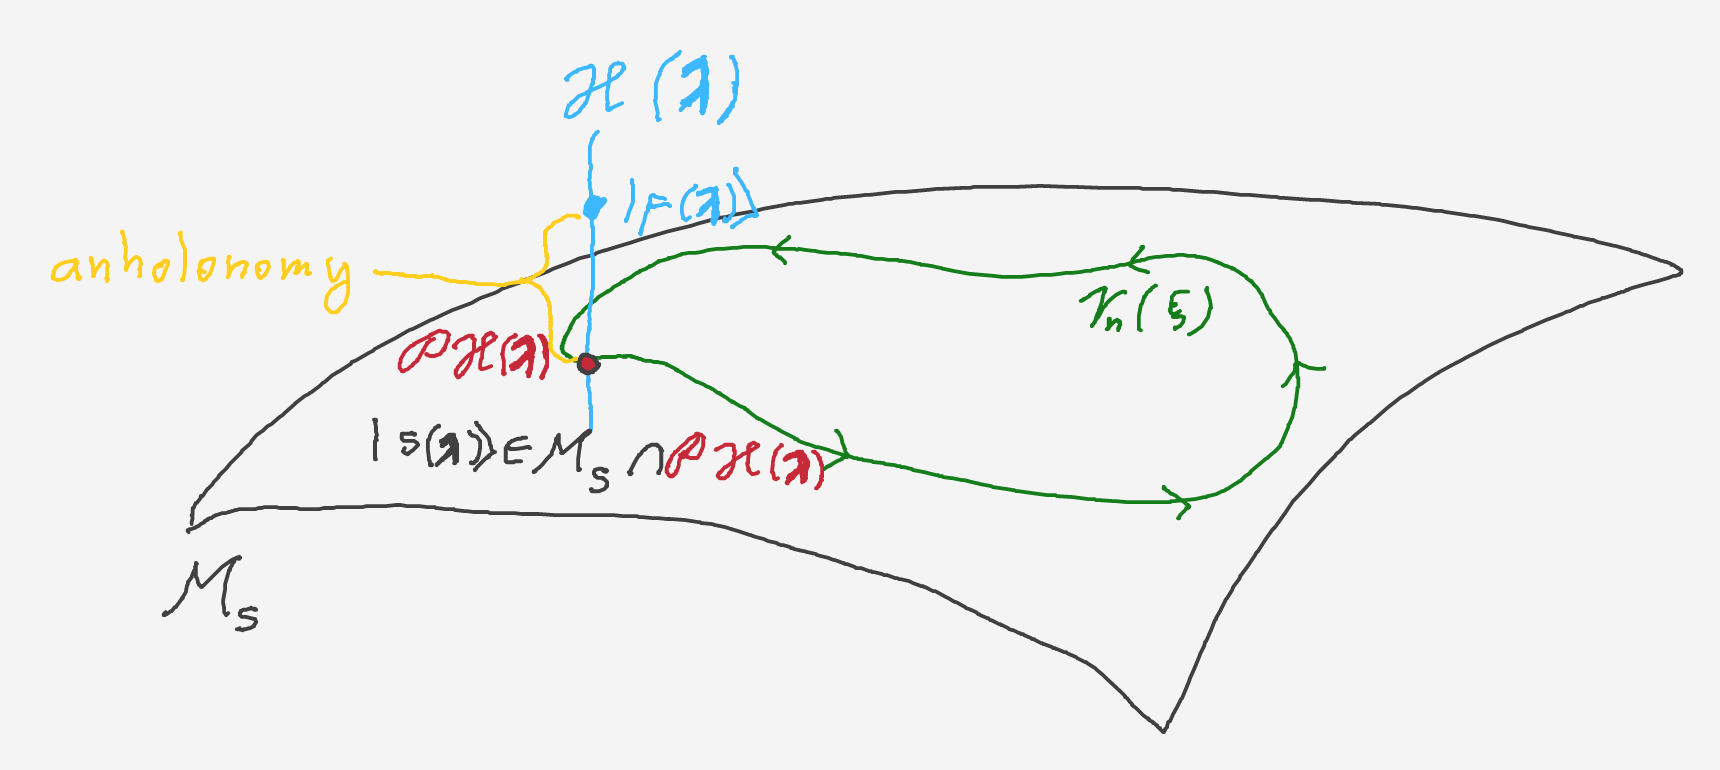
\includegraphics[width=0.8\textwidth]{../img/parallelTransportClosedCurve.png}
\caption{Parallel transporting of states around some closed curve $C$ induces nonzero phase (in geometry angle $\alpha$) between original and transported vector.}
    \label{fig:parallelTransportClosed}
\end{figure}

Substituting general solution \ref{eq:phasesOnManifold} to eq. \ref{eq:schrodinger} yields
\begin{equation}
    \d_t \gamma(t)=i\braket{n(\llambda(t))|\nabla_\llambda n(\llambda(t))}\cdot \d_t \llambda(t).
\end{equation}
Integrating this equation around some closed curve $C$ and assuming the dynamical phase to be zero, thus not exciting the system, we get
\begin{equation}
    \gamma_n(C)=i\oint_C\braket{n(\llambda)|\nabla_\llambda n(\llambda)}\cdot \d \llambda.
    \label{eq:gammaCoint}
\end{equation}
We see, that the geometric phase does not depend on energy or time, only on the sequence of Hamiltonians, which means it depends only on the path itself.




The problem of this expression lies in $\partial_\llambda n(\llambda)$, which locally requires knowledge of single-valued basis $\{\ket{n}\}_n$. This can be avoided in 3-dimensions using Stokes's theorem for $S$ as the surface with boundary $\partial S=C$
\begin{equation}
    \begin{split}
        \gamma_n(C) &= -\Im \iint_C \d S \cdot \nabla \times \braket{n(\llambda)|\nabla n(\llambda)}\\
         &= -\Im \iint_C \d S \cdot \braket{\nabla n(\llambda)|\times|\nabla n(\llambda)}\\
        &= -\Im \iint_C \d S \cdot \sum_{m\neq n} \braket{\nabla n(\llambda)|m(\llambda)}\times \braket{m(\llambda)|\nabla n(\llambda)}\\
        &= -\iint_C \d S \cdot V_n(\llambda)
            \label{eq:stokes}
    \end{split}
\end{equation}
for 
\begin{equation}
    V_n(\llambda) = \Im \frac{
            \braket{n(\llambda)\nabla_\llambda \HH(\llambda) |m(\llambda)}\times \braket{m(\llambda)|\nabla_\llambda \HH(\llambda)|n(\llambda)}    
             }{
(E_m(\llambda)-E_n(\llambda))^2
            }
\end{equation}
where the element of summation $m=n$ in third step of derivation is real, therefore has no influence on $\gamma_n$ and can be omitted. The last equivalence holds, because if we differentiate the \Schrodinger equation \ref{eq:energySchrodinger},  with any covariant derivative $\nabla$, we get 
\begin{equation}
    \begin{split}
        \nabla \HH\ket{n}+\HH \ket{\nabla n} &= E_n\ket{\nabla n}\\
        \braket{m|\nabla \HH|n}+\braket{m|E_m|\nabla n} &= \braket{m|\nabla \HH|n}\\
        \braket{m(\llambda)|\nabla n(\llambda)}&=
        \frac{\braket{m(\llambda)|\nabla \HH |n(\llambda)}}
        { E_m(\llambda)-E_n(\llambda)}, \qquad n\neq m.
    \end{split}
\end{equation}
Comparing the first expression in eq. \ref{eq:stokes} with its last one we see
\begin{equation}
    V_n(\llambda)=\nabla\times\braket{n(\llambda)|\nabla m(\llambda)}, 
    \label{eq:vectorPotentialDef}  
\end{equation}
which defines vector potential of $V_n(\llambda)$. In addition, it extends our definition from single valued basis to any solution of \ref{eq:energySchrodinger}.

As was mentioned, the above procedure from eq. \ref{eq:gammaCoint} was performed only for three dimensional space. Proper generalization to n-dimensional space would yield, see \citep{berry1984},
\begin{equation}
    \gamma_n(C) = -\iint_C \d S \cdot\Im \frac{
            \braket{n(\llambda)\d \HH(\llambda) |m(\llambda)}\wedge \braket{m(\llambda)|\d\HH(\llambda)|n(\llambda)}    
             }{
(E_m(\llambda)-E_n(\llambda))^2
             }.
\end{equation}




\begin{definition}[Adibaticity]
    Slow change in a sense, that it does not excite the system and allows the system to return to the same energetic state after circulation around any closed path on the manifold. For more see Theorem \ref{adiabaticTheorem}.
\end{definition}




\section{Metric and geometric tensor}
Now we need to find some reasonable way to measure the distance on $\M$. Our first guess might be
\begin{equation}
    \d \tilde{s}^2 = \braket{\iota(\bm\llambda+\d\bm\llambda)|\iota(\bm\llambda+\d\bm\llambda)} = 1-2\Re{\braket{\iota(\bm\llambda+\bm\d\llambda)|\iota(\bm\llambda)}}.
\end{equation}
This is \emph{gauge dependent}, meaning that it depends on our choice of the wave phase, i.e. on observer. The phase change $\phi$ induces the change as $\ket{n(\llambda)}\rightarrow e^{i\phi(\llambda)} \ket{n(\llambda)}$, leading to $\braket{n(\llambda)|\nabla n(\llambda)}\rightarrow \braket{n(\llambda)|\nabla n(\llambda)} + i\nabla \phi(\llambda)$. For $\phi(\llambda)\in \mathcal C^2$ we see from eq. \ref{eq:vectorPotentialDef}, that gauge independent choice would be for example 
\begin{equation}
    f=\braket{\iota(\bm\llambda+\d\bm\llambda)|\iota(\bm\llambda)},
\end{equation}
sometimes refered to as the \emph{fidelity}. We can see it's physical meaning imagining \emph{quantum quench} (rapid change of some Hamiltonian parameters), in which case $f^2$ is the probability that system will remain in the new ground state. $1-f^2$ is therefore probability to excite the system during this quench, which leads to the definition of \emph{distance on $\M$}
\begin{equation}
    \d s \equiv 1-f^2= 1-\left|\braket{\iota(\bm\llambda+\d\bm\llambda)|\iota(\bm\llambda)}\right|.
\end{equation}
Using $\d s^2 = g_{\mu\nu}\d \llambda^\mu \d\llambda^\nu+\O(\llambda^3)$, we get the metric tensor
\begin{equation}
    g_{\mu\nu}^{(i)}(\bm\llambda) = \Re\left(\braket{\partial_{\lambda^\mu}\iota(\bm\llambda)|\partial_{\lambda^\nu}\iota(\bm\llambda)} - \braket{\partial_{\lambda^\mu}\iota(\bm\llambda)|\iota(\bm\llambda)}\braket{\iota(\bm\llambda)|\partial_{\lambda^\nu}\iota(\bm\llambda)}\right).
    \label{eq:geom.tensorDefinition}
\end{equation}

Let's have a initial state described by Hamiltonian $\H_\iota=\H(\llambda)$ in eigenstate $\ket{\iota(\llambda)}$, which undergoes the change of parameters $\llambda\rightarrow \llambda+\d \llambda$ resulting in the Hamiltonian $\H_f$ with eigenstates $\ket{\psi_n(\llambda+\d \llambda)}$, $n\in \{1,\dots,dim(\H_f)\}$. Probability amplitude of going to some specific excited state is
\begin{equation}
    \begin{split}
        a_n&=\braket{\psi_n(\llambda+\d\llambda)|\iota(\llambda)}\approx \d\lambda^\mu\braket{\partial_\mu \psi_n(\llambda)|\iota(\llambda} \\
        &= -\d\lambda^\mu\braket{\psi_n(\llambda)|\partial_\mu|\iota(\llambda)}\equiv -\d\lambda^\mu\braket{n|\partial_\mu|\iota},
    \end{split}
\end{equation}
where we introduced shortend notation for eigenstates of the Hamiltonian $\H_0$. If we introduce the \emph{gauge potential}, a.k.a \emph{calibration potential} as
\begin{equation}
    \AA_\mu\equiv i\hbar \partial_{\mu}
\end{equation}
and rescale units to $\hbar=1$, as we will use further on, we get
\begin{equation}
   a_n=\sum_\mu i\braket{n|\AA_\mu |\iota}\d\lambda^\mu,
\end{equation}
which has meaning of matrix elements of the gauge potential. Probability of the excitation i.e. transition to any state $n>0$ is then
\begin{equation}
    \begin{split}
        \sum_{n\neq 0}|a_n|^2&=  \sum_{n\neq 0} \d \lambda^\mu \d \lambda^\nu\braket{\iota|\AA_\mu|n}\braket{n|\AA_\nu|\iota}+\O(|\d \lambda^3|) = \d \lambda^\mu \d \lambda^\nu\braket{\iota|\AA_\mu \AA_\nu|\iota}_c\\
        &= \d \lambda^\mu \d \lambda^\nu\chi_{\mu\nu}+\O(|\d \lambda^3|)=\d s^2+\O(|\d \lambda^3|),
    \end{split}
\end{equation}
where we defined \emph{connected correlation function}, or \emph{covariance}
\begin{equation}
    \braket{\iota|\AA_\mu\AA_\nu|\iota}_c\equiv \braket{\iota|\AA_\mu\AA_\nu|\iota} - \braket{\iota|\AA_\mu|\iota}\braket{\iota|\AA_\nu|\iota}.
    \label{eq:covariance}
\end{equation}
If we leave out $\hbar$, we have the \emph{geometric tensor}\footnote{sometimes defined directly as the expression in eq. \ref{eq:covariance}}
\begin{equation}
    \chi_{\mu\nu}\equiv \braket{\partial_\mu \iota|\partial_\nu \iota}_c = \braket{\partial_\mu \iota|\partial_\nu \iota} - \braket{\partial_\mu \iota|\iota}\braket{\iota|\partial_\nu \iota},
\end{equation}
where $\ket{\partial_\nu \iota}\equiv\partial_\nu \ket{ \iota}$. Because $\chi$ is Hermitian ($\chi_{\mu\nu}=\chi^*_{\nu\mu}$), only the symmetric part adds up to the distance between states 
\begin{equation}
    \d s^2= g_{\mu\nu}\d \lambda^\mu \lambda^\nu= \chi_{\mu\nu}\d \lambda^\mu \lambda^\nu.
\end{equation}
 and only the symmetric part determines the distance between the states. Therefore it's practical to decompose it as
\begin{equation}
    \chi_{\mu\nu} \equiv g_{\mu\nu} - \textcolor{purple}{i\frac{1}{2}} \nu_{\mu\nu},
\end{equation}
where the \emph{Fubini-Study tensor}, as it's called, is
\begin{equation}
    g_{\mu\nu} = \frac{\chi_{\mu\nu}+\chi_{\nu\mu}}{2} = \Re\braket{\partial_\mu i|\partial_\nu i}_c = \textcolor{purple}{\Re \sum_{i\neq j}\frac{\braket{\iota|\pder{\H}{\lambda^\mu}|j}\braket{j|\pder{\H}{\lambda^\nu}|\iota}}{(E_i-E_j)^2}},
    \label{eq:geom.tensorREdefinition}
\end{equation}
and the \emph{curvature tensor} a.k.a. \emph{Berry curvature} is
\begin{equation}
    \begin{split}
        \nu_{\mu\nu} = 2 i(\chi_{\mu\nu}-\chi_{\nu\mu})&= \Im\braket{\iota|[\overleftarrow{\partial}_\nu,\partial_\mu]|\iota}_c = -2 \Im \sum_{i\neq j}\frac{\braket{\iota|\pder{\H}{\lambda^\mu}|j}\braket{j|\pder{\H}{\lambda^\nu}|\iota}}{(E_i-E_j)^2},
    \end{split}
\end{equation}
where $\overleftarrow{\partial}_\nu$ is the derivative of the covector on the left.
Because $g_{\mu\nu}$ is positive semidefinite, it really can be used as the metric tensor.

Fubini-Study tensor can be seen as the Pull-back of the elements of the full Hilbert space to $\M$. 


Next we define the \emph{Berry connection}
\begin{equation}
    A_\mu\equiv \braket{\iota|\AA_\mu|\iota},
\end{equation}
which empovers us to write
\begin{equation}
    \nu_{\mu\nu} = \partial_\mu A_\nu-\partial_\nu A_\mu
\end{equation}
and \emph{Berry phase}
    \footnote{
        The reasonability of this definition can be seen, if we assume the ground state of a free particle
            $\braket{\bm{x}|\iota}=\iota(\bm{x},\llambda)= |\iota(\bm{x})|e^{i\phi(\llambda)}$,
        then the Berry connection is
        \begin{equation}
            A_\mu=-\int \d \bm{x}|\iota|^2\partial_\mu \phi = -\partial_\mu \phi
        \end{equation} 
        and Berry phase
        \begin{equation}
            \phi_B=\oint_\mathcal{C} \partial_\mu \phi \d \lambda^\mu,
        \end{equation}
        which represents total phase accumulated by the wavefunction. It is really the analogy for Berry phase in classical mechanics, which for example for the Faucolt pendulum on one trip around the Sun makes $\phi_B=2\pi$
    }
\begin{equation}
    \phi_B\equiv-\oint_\mathcal{C} A_\mu \d \lambda^\mu=\int_\mathcal{S} F_{\mu\nu}\d \lambda^\mu \wedge \d\lambda^nu,
\end{equation}
where we used the Stokes theorem defining, that the curve $\mathcal{C}$ surrounds some area $\mathcal{S}$.

Wave-functions are elements of the tangent bundle $\TT\in \M$, the gauge potentials are affine connections defining the parallel transport. Covariant derivative is
\begin{equation}
    D_\mu=\partial_\mu+\frac{i}{\hbar}\AA_\mu,
\end{equation}
which yields $D_\mu\ket{\psi_n}=0$ for every eigenstate, which encloses the circle and \textcolor{red}{justifies our initial choise for the distance on $\M$.}








\section{Gauge potentials}
Adiabatic transformation is such a transformation from $\M$ to $\M$, which does not excite the system. Generally it can be achieved by two ways -- infinitely slow transformation of states, or adding some \emph{counterdiabatic elements} to the Hamiltonian to counter the excitation.


In case of adiabatic gauge potential we choose the basis for $\M$ as eigenstates of the Hamiltonian of the full system $\H$. Adiabatic transformation can be understood as parallel transport and adiabatic potentials as affine connection. To understand it more, let's first consider classical system and then move to the quantum mechanics.


\textcolor{blue}{\emph{move elsewhere}: In the case of simple systems, the adiabatic potentials can be found analytically, but for more complicated Hamiltonians we will be forced to use approximations, or some perturbational and variational methods.}




\section{Classical gauge potential}
In the Hamiltonian classical mechanics, we assume the manifold $\M$ \textcolor{red}{to be an accessible part of the phase space} using the Hamiltonian $\H=\H(p_i,q_i)$, where momentum $p_i$ and position $q_i$ are assumed to form the orthogonal basis of the phase space, i.e.
\begin{equation}
    \{q^i,p_j\}=\delta^i_j,
    \label{eq:canonicalCommutationDelta}
\end{equation}
which also defines \emph{calibrational freedom} in their choice. \emph{Canonical transformations} then by definition preserve this formula. Using the \emph{Poisson bracket}, defined as
\begin{equation}
    \{A,B\}\equiv \pder{A}{q^j}\pder{B}{p_j}-\pder{B}{q^j}\pder{A}{p_j},
\end{equation}
we will examine continuous canonical transformations generated by gauge potential $\A_\lambda$
\begin{align}
        q^j(\lambda+\delta\lambda)&=q^j(\lambda)-\pder{\A_\lambda,\bm{p},\bm{q}}{p_j}\delta\lambda \;\Rightarrow\; \pder{q^j}{\lambda}=-\pder{\A_\lambda}{p_j}=\{\A_\lambda,q^j\}
        \label{eq:gaugeAsGeneratorOfMotion1}\\
        p_j(\lambda+\delta\lambda)&=p_j(\lambda)-\pder{\A_\lambda,\bm{p},\bm{q}}{q^j}\delta\lambda \;\Rightarrow\; \pder{p_j}{\lambda}=-\pder{\A_\lambda}{q^j}=\{\A_\lambda,p_j\}.
        \label{eq:gaugeAsGeneratorOfMotion2}
\end{align}
Substituting this to eq. \ref{eq:canonicalCommutationDelta}, we get
\begin{equation}
    \{q^j(\lambda+\delta\lambda),p_j(\lambda+\delta\lambda)\}=\delta^i_j + \mathcal{O}(\delta\lambda^2).
\end{equation}
 
Equations \ref{eq:gaugeAsGeneratorOfMotion1},\ref{eq:gaugeAsGeneratorOfMotion2} are identical to the Hamilton equations
\begin{equation}
\begin{split}
    \dot{q}^j&=-\{\H,q^j\} = \pder{\H}{p_j}\\
    \dot{p}_j&=-\{\H,p_j\} = -\pder{\H}{q^j},
\end{split}
\end{equation}
if $\A_t=-\H$. Because the Hamiltonian is generator of the movement in the phase space $(\bm{q},\bm{p})$, we can interpret $\A_t$ as the generators of the movement on $\M$. Specially if we chose $\lambda=X^i$, we get $\A_{X^i}=p_i$.




\section{Quantum gauge potential}
\citep{kolodrubez}[kap. 2.2]
The role of Poison brackets in quantum mechanics is taken by commutators, canonical transformations are called \emph{unitary transformations} and calibrational freedom is hidden in the choice of basis. We can write the unitary transformation $\U$ between initial system $S$ and the transformed $\tilde{S}$ along some path on $\M$ defined by eigenstates $\{\ket{m(\llambda)}\}_m$. Let the initial state be $\kpsi$ and define unitary transformation
\begin{equation}
    \U(\llambda)^+: \kpsi \rightarrow \ket{\tilde\psi(\llambda)},
    \label{eq:transformationU}
\end{equation}
which satisfies
\begin{equation}
    i\hbar \partial_\lambda \U(\lambda)=\HH(\lambda)\U(\lambda)
\end{equation}
The wavefunction $\kpsi$ in $S$ can be decomposed using Schmidt decomposition\footnote{The Schmidt decomposition can be performed in finite dimension, or if the Hamiltonian is compact, which is not automatic in quantum mechanics. What's more, the Hamiltonian is usually not even bounded. Anyway, for simple systems with bounded energy we can assume so.}, as
\begin{equation}
    \kpsi = \sum_{m,n}\psi_n \U_{nm}^*\ket{m(\llambda)} = \sum_m \overbrace{\tilde{\psi}_m(\llambda)}^{\braket{m(\llambda)|\psi}}\ket{m(\llambda)}.
\end{equation}
We can define adiabatic potentials analogically to the classical case as
\begin{equation}
    i\hbar\partial_\lambda \ket{\tilde{\psi}(\llambda)} = i\hbar \partial_\lambda\left(\U^+(\llambda)\ket{\psi} \right)= \underbrace{i\hbar\left(\partial_\lambda \U^+(\llambda)\right)\U(\llambda)}_{-\tilde{\AA_\lambda}}\ket{\tilde{\psi}(\llambda)},
\end{equation}
which can be transformed to non-tilde system as
\begin{equation}
    \begin{split}
        \AA_\lambda&=\U(\llambda)\tilde{\AA_\lambda}\U^+(\llambda) = -i\hbar\big(\U(\llambda)\partial_\lambda \U^+(\llambda)\big) =\\
        &= -i\hbar\big(\partial_\lambda(\underbrace{U^+(\llambda)U(\llambda)}_{\mathds{1}})-\partial_\lambda(U(\llambda))U^+(\llambda) \big) =i\hbar \big(\partial_\lambda U(\llambda))U^+(\llambda).
    \end{split}
\end{equation}
Thus we get equations for adiabatic potentials
\begin{align}
    \AA_\lambda&=i\hbar \big(\partial_\lambda U(\llambda))U^+(\llambda)
    \label{eq:adiabaticPotential}\\
    \tilde{\AA_\lambda} &= -i\hbar\left(\partial_\lambda \U^+(\llambda)\right)\U(\llambda)
    \label{eq:adiabaticPotentialTilde}
\end{align}
These potencials are Hermitean (omitting referrence to $\llambda$ in brackets)
\begin{equation}
     \tilde{\AA_\lambda}^+=i\hbar U^+\partial_\lambda\U=-i\hbar\partial_\lambda\U^+\U = \tilde{\AA_\lambda} ,
\end{equation}
analogically holds for $\AA_\lambda$ and using the eigenbasis of $\HH$, the matrix elements are
\begin{equation}
    \bra{n}\tilde{\AA_\lambda}\ket{m}=i\hbar\bra{n}\U^+\partial_\lambda\U\ket{m} = i\hbar\bra{\tilde n(\lambda)}\partial_\lambda\ket{\tilde m(\lambda)}.
\end{equation}
and because
\begin{equation}
    \bra{\tilde n(\lambda)}\AA_\lambda\ket{\tilde m(\lambda)}= \bra{n}\tilde{\AA_\lambda}\ket{m},
\end{equation}
we get
\begin{equation}
    \A_\lambda = i\hbar\partial_\lambda.
    \label{eq:adiabaticPotentialDefinition}
\end{equation}
It's good to point out, that we were applying tilde operators to non-tilde states et vice versa. This can be justified only if we consider $\M$ big enough to contain all necessary states, which can be achieved during the transformation.


According to eq. \ref{eq:phasesOnManifold}, $\U$ can be explicitly chosen as
\begin{equation}
    \U(t)=\sum_n \exp\left(\frac{i}{\hbar}E_n(\tau)\d \tau - \int_0^t \braket{n(\tau)|\partial_\tau n(\tau)}\d\tau\right)\ket{n(t)}\bra{n(0)}.
\end{equation}
This was not needed for the derivation of the adiabatic element, but gives us explicit formula for.............

\section{Adiabatic transformations}
In this chapter, we will be dealing with the system described by finite-dimensional Hamiltonian $\HH=\HH(\llambda)$ which drives the system according to \Schrodinger equation from some initial state $\ket{n(\llambda(0))}$ to $\ket{n(\llambda(t))}$. The action minimization theorem states, that there exists some path minimizing action, which allows us to reduce the dimension of $\M$ from the $\R^n$ to $1$ using parametrisation $\gamma(\lambda)$, so we get $\HH=\HH(\lambda)$.

\subsection{Adiabatic potential}
Important knowledge about symmetries of the system is encoded in canonical transformations, or in quantum mechanics more commonly referred to as \emph{unitar transformations}. In our case, the generators of such canonical transformations are adiabatic potentials. In case of the Hamiltonian $\H(\llambda)$ and it's adiabatic transformation $\H(\llambda+\d \llambda)$, we get
\begin{equation}
    [\HH(\llambda),\HH(\llambda+\d \llambda)]=0,
\end{equation}
meaning Hamiltonian commutes with it's canonically transformed version.\footnote{This can be easily reformulated to the world of classical physics, where the commutator is replaced by Poisson bracket.}


\subsection{Adiabatic transformation}
\citep{kolodrubez}[chap. 2.3]
As was mentioned in the introduction to this chapter, one way to change the system parameters without exciting it is to change the driving parameter slowly enough. The meaning of the word "slow" clears up next theorem.
\begin{thm}[Adiabatic theorem]
    \label{adiabaticTheorem}
    For Hamiltonian $\HH$ varying in the time range $T$, the solution of the Schrödinger equation 
    $$\HH(t)\ket{\psi_n(t)} = E_n(t)\ket{\psi_n(t)}$$
    with initial condition in x-representation $\braket{x|\psi(t=0}=\psi_n(x,0)$ can be approximated as
    \begin{equation}
      ||\psi(t) - \psi_{ad}(t)||\approx o\left(\frac{1}{T}\right)
    \end{equation}
    for \emph{adiabatic state}
    \begin{equation}
        \ket{\psi_{ad}}= e^{\theta_n(t)}e^{\gamma_n(t)}\ket{\psi(t)},
    \end{equation}
    where we define \emph{nongeometrical phase} induced by energy transitions,
    $$\theta_n(t)\equiv -\frac{1}{\hbar}\int_0^t E_n(\tau)\d \tau$$
    and \emph{geometrical phase}, also called \emph{Berry phase}
        $$\gamma_n(t)\equiv \int_0^t \underbrace{i\braket{\psi_n(\tau)|\partial_\lambda\psi_n(\tau)}}_{\nu_n(\tau)} \d \tau .$$
\end{thm}
\begin{myproof}
    TBD (na wiki je)
\end{myproof}
Assume differentiable and non-singular Hamiltonian $\HH(\llambda)$ with degenerate basis $\{\ket{m,\llambda}\}_m$ called the \emph{adiabatic basis}. This is generally the family of adiabatically connected eigenstates\footnote{In the case of energy level crossing, the eigenstates are not unified, because transition between them is not adiabatical.} The transition amplitude between states for adiabatic change is
\begin{equation}
    0=\bra{m}\HH\ket{n} \quad \text{pro }n\neq m.
\end{equation}
This can be driven along some curve $\gamma(\lambda)$, i.e. differentiated by $\partial_\lambda$:
\begin{equation}
    \begin{split}
        0&=\bra{\partial_\lambda m}\HH\ket{n}+ \bra{m}\partial_\lambda\HH\ket{n}+ \bra{m}\HH\ket{\partial_\lambda n}\\
        &=E_n\braket{\partial_\lambda m|n} + E_m\braket{m|\partial_\lambda n}+ \bra{m}\partial_\lambda \HH\ket{n}\\
        &= (E_m-E_n)\underbrace{\braket{m|\partial_\lambda n}}_{-\frac{i}{\hbar}\bra{m}\AA_\lambda\ket{n}} + \braket{m|\partial_\lambda\HH|n},
    \end{split}
\end{equation}
where $\HH$, $\ket{n}$, $\ket{m}$ and $E_n$ are functions of $\lambda$.

In matrix form, we can rewrite this equation as
\begin{equation}
    i\hbar\partial_\lambda\HH=[\AA_\lambda,\HH]-i\hbar \hat{M}_\lambda\qquad \text{for } \hat{M}_\lambda\equiv -\sum_n\pder{E_n(\lambda)}{\lambda}\ket{n(\lambda)}\bra{n(\lambda)}.
\end{equation}
$\hat{M}$ is diagonal in energetic basis and it's elements has meaning of \emph{generalized force}, which correspond to corresponding energetic states. We can easily see that $[\HH,\hat{M}]=0$, implying
\begin{equation}
    [\HH,i\hbar\partial_\lambda\HH-[\AA_\lambda,\HH]]=0.
    \label{eq:komutation}
\end{equation}
This can be used as the definition for \emph{counterdiabatic potential} $\AA_\lambda$. The strength of this equation lies in the fact, that it finds counterdiabatic potential without the need of Hamiltonian diagonalisation.

\section{Counterdiabatic driving}
\citep{kolodrubez}[page 15--17]
Again consider two bases consisting of eigenstates of Hamiltonian $\HH=\HH(\lambda(t))$. $B(t)$ for external observer and $\tilde B(t)$ for frame activelly transformed by Hamiltonian (moving frame), in which $\tilde \HH(t)$ is diagonal. Transforming vectors in Schrödinger equation
\begin{equation}
    i\hbar \der{}{t}\ket{\psi(t)} = \HH(\lambda(t))\ket{\psi(t)}
\end{equation}
to moving frame using unitary operator for time varying Hamiltonian (compare to eq. \ref{eq:transformationU}
\begin{equation}
    \U(\lambda(t)): \ket{\tilde\psi(\lambda(t))} \rightarrow \ket{\psi(t)}.
    \label{eq:transformationUtimeDependentH}
\end{equation}
and using \emph{dot} notation for time derivative, we get
\begin{align}
    i\hbar \der{}{t}(\U\ket{\tilde \psi}) &= \HH\U\ket{\tilde \psi} \\
    i\hbar \dot \lambda\partial_\lambda\U\ket{\tilde \psi} + i\hbar \U\der{}{t}\ket{\tilde \psi} &= \HH\U\ket{\tilde \psi}.
\end{align}
This can be rewritten using adiabatic potential from eq. \ref{eq:adiabaticPotentialDefinition}) as
\begin{equation}
    i\hbar \der{}{t}\ket{\tilde{\psi}} = \left[\U^+\HH\U-\dot{\lambda}\tilde{\AA_\lambda}\right]\ket{\tilde{\psi}} = \left[\tilde \HH-\dot{\lambda}\tilde{\AA_\lambda}\right]\ket{\tilde{\psi}} = \tilde{\HH}_m \ket{\tilde{\psi}}.
\end{equation}
Hamiltonian in moving frame is $\tilde\HH(t)=\U^+(\lambda(t))\HH(\lambda(t))\U(\lambda(t))$ and the term $-\dot{\lambda}\tilde{\AA_\lambda}$ is called \emph{Galilean}. To Hamiltonian in moving frame $\HH_m = \HH-\dot{\lambda}\AA_\lambda$ we can add \emph{counterdiabatic element} $\dot{\lambda}\AA_\lambda$ and the only remaining element is $\HH$, which does not excite the system.

\section{Approximations of adiabatic potentials}
Adiabatic potentials can be calculated from the principal of minimal action, which leads to variational method.

If the difference between eigenstates of $\HH$ is small, or generalized force between some states is zero, the computation of the adiabatic potential is numerically unstable. The knoledge of exact adiabatic potential would allow to maintain the system in the ground state thus not exciting it, as th Eigenstate thermalization hypotheses states.

\begin{hypot}[Eigenstate thermalization hypotheses]
  For the difference between eigenstates of $\HH$ and extensive thermodynamic entropy $S$, it holds that
    \begin{equation}
    E_n-E_m\propto \exp\left(\frac{S}{2}\right).
  \end{equation}
  If the states are close, better approximation would be $E_n-E_m\propto \exp(S)$. For matrix elements it holds, that they vanish exponentially with the characteristic scale of the system $a$, i.e.
  \begin{equation}
    \bra{m}\AA_\lambda\ket{n} = i\hbar\frac{\braket{m|\partial_\lambda \HH|n}}{E_m-E_n} \propto \exp(-a).
    \label{eq:thermalizationMatrixElements}
\end{equation}
\end{hypot}
Fortunatelly in the limit "number of particles" $\rightarrow \infty$ the expression in eq. \ref{eq:thermalizationMatrixElements} converges.

\subsection{Variational methods}
